\section{Experiments}







\subsection{Experimental Setup}







\paragraph{Models.}
We use GPT-2 \citep{radford2019language}, GPT-3 \citep{Brown2020LanguageMA}, and GPT-Neo \citep{gpt-neo} models. The GPT architecture is especially appropriate for text generation because it is autoregressive. However, GPT-2 was not pretrained on code, so we pretrain it on GitHub as described in the next paragraph. Anecdotal evidence indicates that GPT-3 can generate code. To determine the extent of its code generation ability, we use the `davinci' (Instruct series) model, the largest publicly available model speculated to have 175 billion parameters. Finally, GPT-Neo has an architecture similar to GPT-3, and it was pretrained on the Pile \citep{gao2020pile} which includes GitHub. Unlike GPT-3, GPT-Neo's weights are publicly available, hence we are able to fine-tune it with APPS.






\paragraph{GPT-2 Pretraining.}
Since GPT-2 was trained on natural language and not code, we collected GitHub code to further pretrain GPT-2. GitHub repositories with fewer than one star were filtered out.
While Neo's GitHub pretraining data did \emph{not} undergo an APPS data decontamination process, our GPT-2 models are trained on decontaminated data.
Specifically, all repositories matching certain keywords that would suggest overlap with common programming exercises were removed. We provide the list of keywords in the Supplementary Materials. We also discard any GitHub code that contains functions with the same signatures as functions in the starter code in many of our APPS problems. This leaves us with 30 GB of Python code. To improve the efficiency of pretraining, we process all Python code in the pretraining dataset by converting from spaces to tabs, which saves the character conversion when running model tokenizers.



\paragraph{Fine-tuning.}
During fine-tuning with APPS, the objective is to predict the entire code solution, given both the English text problem statement and the problem format (call-based format or standard input format). For problems with starter code, we exclude the starter code from the training loss.


Across pretraining and fine-tuning, we use the AdamW optimizer \citep{Loshchilov2019DecoupledWD}, a batch size of $256$, and a weight decay of $0.05$. We fine-tune for $10$ epochs. We use DeepSpeed and its implementation of the ZeRO optimizer to reduce memory consumption while training large models \citep{Rasley2020DeepSpeedSO, rajbhandari2020zero}. Unless otherwise specified, we use the default HuggingFace generation parameters, except that we use beam search with a beam size of $5$. Models are fine-tuned on 8 A100 GPUs.


\subsection{Metrics}
To obtain a comprehensive evaluation of code generation ability, we use the large bank of test cases and ground-truth solutions provided with APPS. Test cases allow for \emph{automatic} evaluation, even though the the space of possible programs can be combinatorially large. Therefore, unlike many other text generation tasks, manual analysis is not necessary. We aggregate the generated code's performance on test cases with two metrics, ``test case average'' and ``strict accuracy.'' %

\textbf{Test Case Average.}\quad We compute the average fraction of test cases passed. 
Concretely, let the number of problems in the test set be $P$. For a given problem $p$, let the code generated to solve problem $p$ be denoted $\langle\texttt{code}_p\rangle$, and set of test cases for problem $p$ be $\{(x_{p,c},\, y_{p,c})\}_{c=1}^{C_p}$. Then the test case average is 
\[
\frac{1}{P}\sum_{p=1}^P \frac{1}{C_p} \sum_{c=1}^{C_p} \mathds{1}\{\texttt{eval}(\langle\texttt{code}_p\rangle,x_{p,c}) = y_{p,c}\}.
\]

Oftentimes, solutions can successfully pass a subset of the test cases but not cover every corner case. This allows for less stringent model evaluation, as strict accuracy may currently obscure model improvements.

\begin{table*}[t]
\setlength{\tabcolsep}{2pt}
\small
\centering
\begin{tabular}{lcccc|cccc}
\multicolumn{1}{l}{} &  \multicolumn{4}{c}{Test Case Average} & \multicolumn{4}{c}{Strict Accuracy} \\
Model       & Introductory & Interview & Competitive &  Average & Introductory & Interview & Competition &  Average \\

\toprule
GPT-2 0.1B          & 5.64 & 6.93 & 4.37 & 6.16 & 1.00 & 0.33 & 0.00 & 0.40 \\
GPT-2 1.5B          & 7.40 & 9.11 & 5.05 & 7.96 & 1.30 & 0.70 & 0.00 & 0.68 \\
GPT-Neo 2.7B        & 14.68 & 9.85 & 6.54 & 10.15 & 3.90 & 0.57 & 0.00 & 1.12 \\
GPT-3 175B        & 0.57 & 0.65 & 0.21 & 0.55 & 0.20 & 0.03 & 0.00 & 0.06 \\
\end{tabular}
\caption{Average percentage of test cases passed and strict accuracy for each model and difficulty level. All values are percentages. Note `0.1B' indicates the number of model parameters in billions. GPT-3 is a \emph{few-shot} model and not fine-tuned, unlike the other models. GPT-Neo does best and attains approximately 4\% strict accuracy on Introductory problems, and for these problems it passes approximately 15\% of the test cases.}
\label{tab:results}
\end{table*}

\textbf{Strict Accuracy.}\quad Eventually, generated solutions should pass all test cases including corner cases.
To compute the strict accuracy which requires programs pass every test case, we run the code generated by the model on every test case of every problem. Strict accuracy is then computed by taking the number of solutions passing every test case divided by the total number of exercises. Using the notation from before, we can write the strict accuracy as $\frac{1}{P}\sum_{p=1}^P \prod_{c=1}^{C_p} \mathds{1}\{\texttt{eval}(\langle\texttt{code}_p\rangle,x_{p,c}) = y_{p,c}\}.$ Future research may only use strict accuracy when models become sufficiently capable.


\subsection{Model Performance Analysis}

\paragraph{Qualitative Output Analysis.} Models can sometimes generate correct or superficially plausible code. \Cref{fig:samples_from_1500} shows code generated by GPT-2 1.5B that passes all test cases. When models do not pass the test cases, sometimes their generated code still appears plausible at first glance. For example, in \Cref{fig:interesting_sample_from_1500}, we see that the 1.5B parameter model generates code that is related to the problem statement and makes a plausible attempt to solve it.


\paragraph{Test Case Evaluation.}
We show the main results in \Cref{tab:results}. We observe that models are able to generate code that passed some test cases, implying many generated programs are free of syntax errors and can successfully process inputs test cases to produce correct answers. Note that for Introductory questions, GPT-Neo passes approximately $15\%$ of the test cases. We visualize Test Case Average results in \Cref{fig:partial}. This demonstrates models are showing marked improvements on code generation and now starting to have traction on code generation.

\begin{wraptable}{r}{0.43\textwidth}
\begin{center}
\begin{tabular}{l|cc}
    & Top-1 & Top-5 \\ \midrule
Test Case Average & $14.7\%$ & $19.9\%$ \\
Strict Accuracy & $3.9\%$ & $5.5\%$ \\
\bottomrule
\end{tabular}
\caption{GPT-Neo 2.7B performance on introductory problems using one generated program (Top-1) and the best of five generated programs (Top-5). Full results are in the Supplementary Materials. %
}
\label{tab:topk}
\end{center}
\end{wraptable}

Performance can be further improved by sampling multiple solutions and selecting the best. Here, we perform beam search with beam width $5$ and evaluate its $5$ beams, so that each model has five attempts to get a problem correct rather than one. With this setup, GPT-Neo's strict accuracy on Introductory problem then exceeds $5\%$, as shown in \Cref{tab:topk}. Our results in the Supplementary Materials show that the top-5 test case average GPT-2 0.1B is 10.75 while the top-1 test case average of GPT-2 1.5B is 7.96. This highlights that simply sampling multiple candidate solutions is a powerful way to markedly improve performance.

Our results also provide us with information about the importance of model choice. Evidently existing few-shot GPT-3 models are not necessarily better at code generation than fine-tuned models that are smaller by two orders of magnitude. Additionally, performance improvement from GPT-2 1.5B to GPT-Neo 2.7B is larger than that from GPT-2 0.1B to GPT-2 1.5B. Potential causes of GPT-Neo's better performance are that GPT-Neo is trained on more code from GitHub, it has more parameters, or its architecture hyperparameters were chosen better. Memorization explaining all performance is an implausible explanation as performance tracks problem difficulty; were models just memorizing, we would expect uniform performance across difficulties. Since models still have large room for improvement, solving the APPS benchmark without unreasonable amounts of computational resources may require architectural or algorithmic improvements.

\paragraph{Syntax Errors.} We now assess the frequency of syntax errors, errors that prevent the program from being interpreted including inconsistent spacing, unbalanced brackets, missing colons, and so on. Syntax errors are identified in our testing framework based on the heuristic of whether pyext is able to load the generated code as a Python module. For our purposes, this almost exclusively occurs for syntax errors. We visualize the prevalence of syntax errors in \Cref{fig:syntax}. While approximately $59\%$ of GPT-3's generated solutions for introductory problems have syntax errors, GPT-Neo syntax error frequency is approximately $3\%$. Note that recent work such as \cite{Yasunaga2020GraphbasedSP} create a separate model to repair source code to fix compilation issues, but our results suggest that such efforts may be unnecessary in the future as syntax error frequency is sharply decreasing automatically.


\begin{figure}[t]
\begin{minipage}{.49\textwidth}
\centering
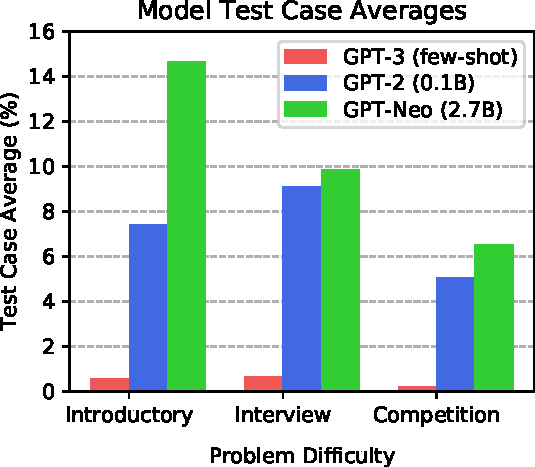
\includegraphics[width=\textwidth]{figures/partial_credit.pdf}
\caption{The average percentage of test cases passed increases with larger fine-tuned models.%
}\label{fig:partial}
\end{minipage}\hfill%
\begin{minipage}{.49\textwidth}
\centering
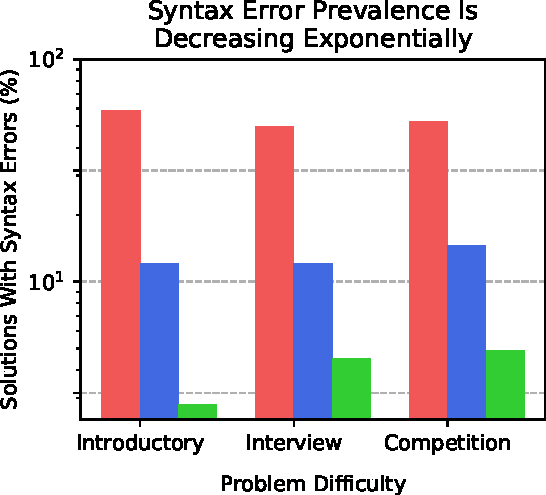
\includegraphics[width=\textwidth]{figures/syntax_issues.pdf}
\caption{Syntax errors decrease exponentially with fine-tuning and increased model sizes. GPT-Neo 2.7B has very few syntax errors.}\label{fig:syntax}
\end{minipage}
\end{figure}

\paragraph{BLEU.} We find that assessing model performance with BLEU is a poor substitute for evaluating with test cases. To evaluate BLEU, we take the generated solution and compute its BLEU with each human-written solution for a given problem; we then record the highest BLEU score. Observe in \Cref{fig:bleu} that BLEU increases as problem sources become more difficult, even though models actually perform worse on harder problems. Moreover, worse models can have similar or higher BLEU scores. For example, GPT-2 0.1B has $26.8$, $29.7$, and $30.2$ as BLEU scores for introductory, interview, and competition problems, respectively. Meanwhile GPT-Neo 2.7B has $27.1$, $29.1$, and $29.3$ as its BLEU scores, respectively. Hence BLEU wrongly suggests GPT-Neo is a worse model. 











\begin{wrapfigure}{r}{0.5\textwidth}
    \centering
    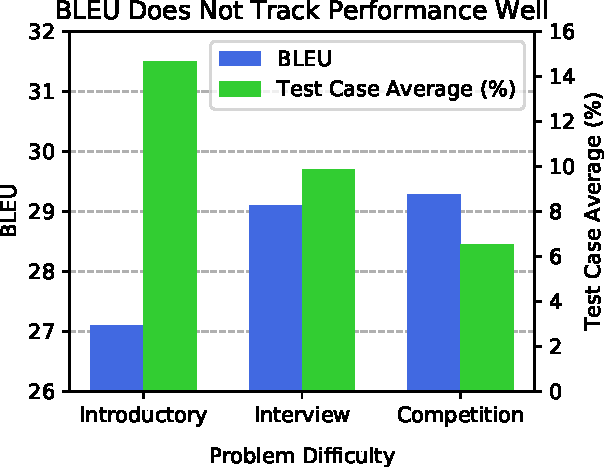
\includegraphics[width=0.5\textwidth]{figures/bleu.pdf}
    \caption{BLEU scores for GPT-Neo 2.7B increase with difficulty level and are anticorrelated with a gold-standard accuracy metric.}
    \label{fig:bleu}
\end{wrapfigure}

\paragraph{Evaluating GPT-3.}
We evaluate GPT-3 175B on APPS in a few-shot setting. A separate prompt is used for standard input and call-based questions, and each prompt includes instruction text along with two example questions and solutions from the corresponding question type. We find that GPT-3 only solves $3$ problems out of $5,\!000$: two introductory problems and one interview problem. The two introductory problems are simple interpretation tasks, such as implementing a specified algebraic expression. The interview problem requires higher-level thinking that suggests nontrivial reasoning. However, it is possible that GPT-3 memorized the solution during pretraining, or that it took a lucky guess based on heuristics in the question. One potential factor in GPT-3's poor performance is that it handles syntax poorly. Namely, we observed cases where improper formatting of otherwise functioning code causes a syntax error. For specific examples and more details, see the Supplementary Materials.

\paragraph{Evaluations on Larger Models.}
Since the public release of APPS, several others have trained even larger models on APPS than we evaluate here. OpenAI Codex is a 12B parameter Transformer language model pre-trained on large quantities of public code and comments. \citet{chen2021evaluating} evaluate Codex on APPS under various configurations and achieve top-1 and top-5 accuracy on introductory problems of 4.14\% and 9.65\% respectively, close to double the top-5 accuracy of GPT-Neo 2.7B. Furthermore, by scaling up to a top-1000 evaluation they obtain 25\% accuracy. This demonstrates that larger models trained specifically for code generation can improve APPS performance even further, but are still far from solving the task.